\documentclass[11pt]{article}
\usepackage{graphicx}
\usepackage{titling}
\usepackage{geometry}
\graphicspath{ {./images/} }

\author{Chad Lape and Colton Murray}
\title{Lab 2 Report}
\date{\today}
\setlength{\droptitle}{-4em}

\begin{document}

\maketitle

\section{Objectives}
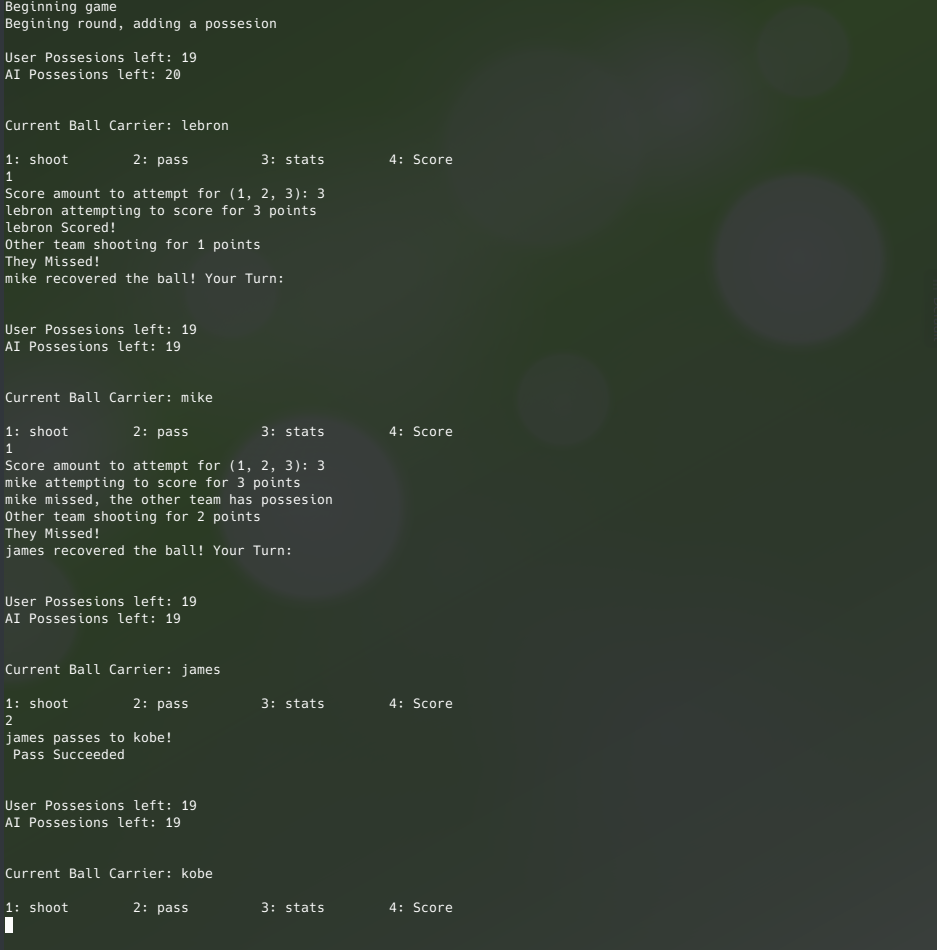
\includegraphics[scale=0.5]{pic.png}\\
This task involved the creation of a class and implementation of that class as an object within a larger code. This is one of the fundamental concepts of modern computing; object oriented programming. This is due to Object Oriented Programming being able to combine together data and functionality and helps to specify the uses of different data. 

\section{Public and Private Data}
\subsection{Private Variables}
\begin{itemize}
\item name
\item shotsTaken
\item shotsAttempted
\item passesAttepted
\item passesMade
\end{itemize}
All of these variables are data base data which must be derived from memory or files. Thus they can be private and used with member functions; this ensures the information is not misused and will act in more predicatable ways.

\subsection{Public Members}
\subsubsection{Constructor}
\begin{itemize}
\item Player(string);
\end{itemize}
This will just start the player with a string and with a randomized shots made/attempted and passes made/attempted; this is to ensure each game is different
\subsubsection{Setters/Getters}
\begin{itemize}
\item 	void setName(string);
\item 	string getName() {return name;}
\item 	int getshotsTaken();
\item 	void setshotsTaken(int);
\item	int getshotsMade();
\item	void setshotsMade(int);
\item	int getpassesAttempted();
\item	void setpassesAttempted(int);
\item	int getpassesMade();
\item	void setpassesMade(int);
\end{itemize}
These all involve interacting with the private variables. This allows for them to act in more specific ways and sometimes force the 
\subsubsection{Member Functions}
\begin{itemize}
\item	bool passBall();\\
Will attempt a pass and return a boolean of whether the player made or failed the pass. Will also iterate the pass private variable accordingly
\item	int takeShot(int);\\
Will attempt to make a shot and return the score if it was successful or zero if it was not. This is then handled within the main file by using the data returned for updating the state of the game.
\item	void getStats();\\
Prints the stats of the player as well as their name. Does not return as that was not needed in this program and only needed to print.
\end{itemize}



\end{document}